In this section we demonstrate the methods described so far and implemented in the software using a simple scenario. The network, shown in Figure \ref{fig:config}, has six links numbered 0 through 5. Links 0 through 4 have flow capacities of 2,000 veh/hour, while link 5 has a capacity of 1,00 veh/hour. All links except for link 2 are 200 meters in length. Link 2 is 400 meters. The free-flow speed in all links is 70 km/hr, and hence the free-flow travel time for all links except link 2 is about 10 seconds, while for link 2 it is about 20 seconds. There are two origin/destination pairs: OD 1, going from source node 0 to sink node 5, and OD 2, going from source node 1 to sink node 5. There are two paths available to OD 1: path 1, consisting of links [0, 3, 4, 5], and path 2 consisting of links [0, 2, 4, 5]. OD 2 is confined to path 3 = [1, 3, 4, 5]. Path [1, 2, 4, 5] is not utilized.

\begin{figure}[h]
    \centering
    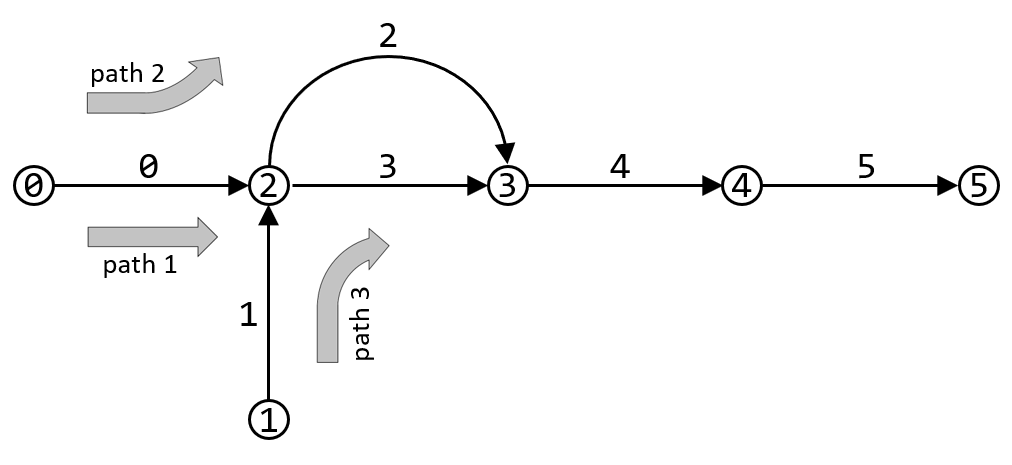
\includegraphics[width=\linewidth]{figs/config.png}
    \caption{Traffic network.}
    \label{fig:config}
\end{figure}

\subsection{Static assignment}
The static assignment problem is the simplest form of traffic assignment. It is posed with the static model and travel time functions of Eqs. \XXX and \XXX, and solved with the Frank-Wolfe algorithm. Figure \XXX shows solutions to the problem with $\gamma$ ranging fro $\XXX$ to $\XXX$. The plot shows that the demand assigned to path 1 is inversely proportional to the logarithm of $\gamma$. 
 
The demands for the two OD pairs are $d_0 = 200$ veh/hour and $d_1=400$ veh/hour for \XXX minutes. Thus, the capacity of link 4 is exceeded by 100 veh/hour. Beyond the \XXX th minute, all demands are set to zero. Because OD 1 has only one available path, the traffic assignment problem consists simply in deciding, at each time step, how to split $d_0$ amongst paths 1 and 2. 

Figure \XXX shows the result of the traffic assignment calculation using the static model with BPR coefficients selected according to the link capacities and lengths. The result was obtained using the Frank-Wolfe algorithm, which ran for \XXX iterations and completed in a negligible amount of time. 

DESCRIBE THIS RESULT

Figure \XXX shows the equilibrium solution under the MN model. This solution was computed using the \XXX algorithm, and completed after \XXX iterations (~\XXX seconds)

DESCRIBE THE RESULT

Figure \XXX shows the equilibrium solution under the CTM model and both instantaneous and predictive travel time. This solution was computed using the \XXX algorithm, and completed after \XXX iterations (~\XXX seconds)

QUALITATIVE COMPARISON OF THE RESULTS.


\begin{figure}[h]
    \centering
    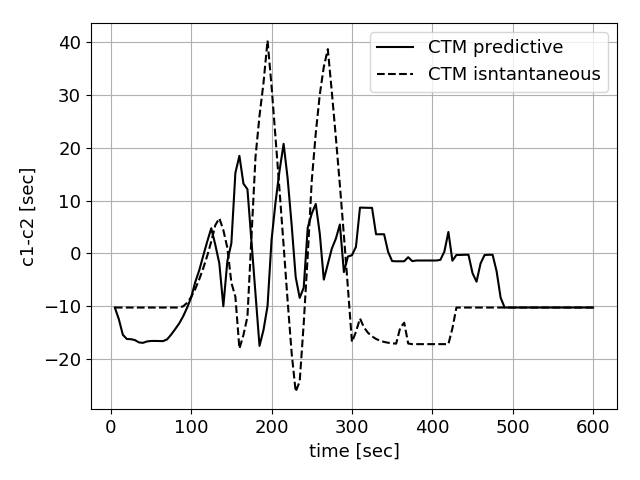
\includegraphics[width=0.9\linewidth]{figs/cdiff_1300.png}
    \caption{\XXX }
    \label{fig:cdiff}
\end{figure}

\begin{figure}[h]
    \centering
    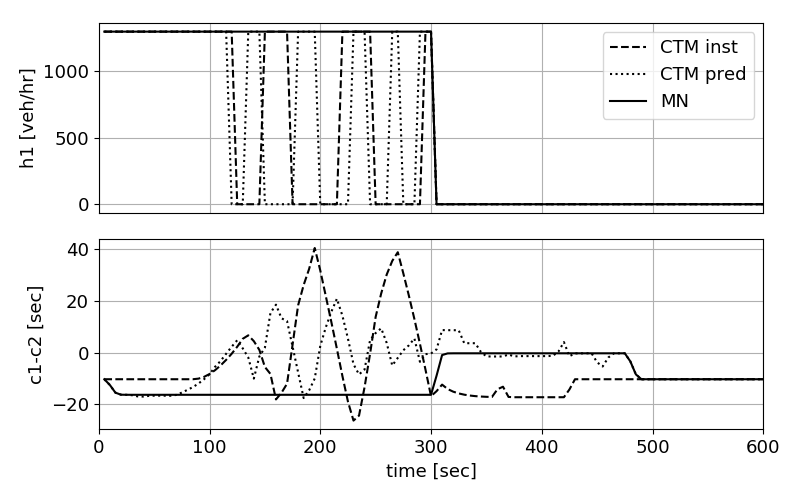
\includegraphics[width=\linewidth]{figs/ctm_vs_mn_hc.png}
    \caption{\XXX }
    \label{fig:ctm_vs_mn_hc}
\end{figure}

\begin{figure}[h]
    \centering
    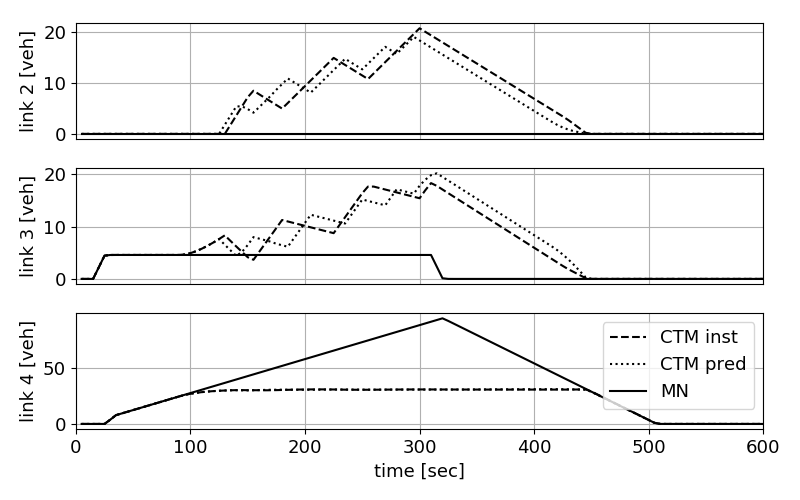
\includegraphics[width=\linewidth]{figs/ctm_vs_mn_x.png}
    \caption{\XXX }
    \label{fig:ctm_vs_mn_x}
\end{figure}

\begin{figure}[h]
    \centering
    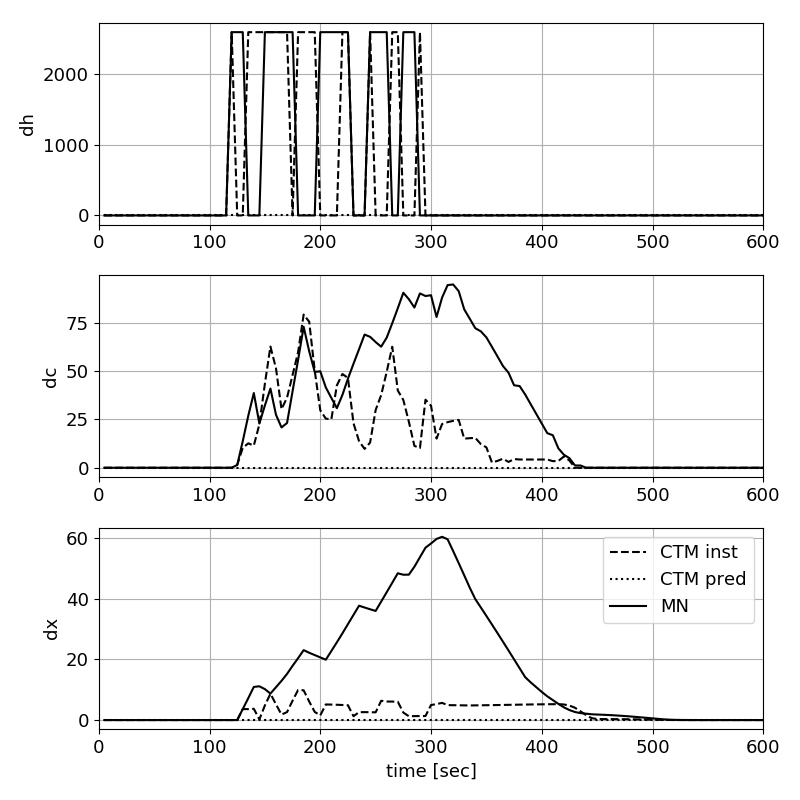
\includegraphics[width=\linewidth]{figs/dist2ctm.png}
    \caption{\XXX }
    \label{fig:dist2ctm}
\end{figure}

\begin{figure}[h]
    \centering
    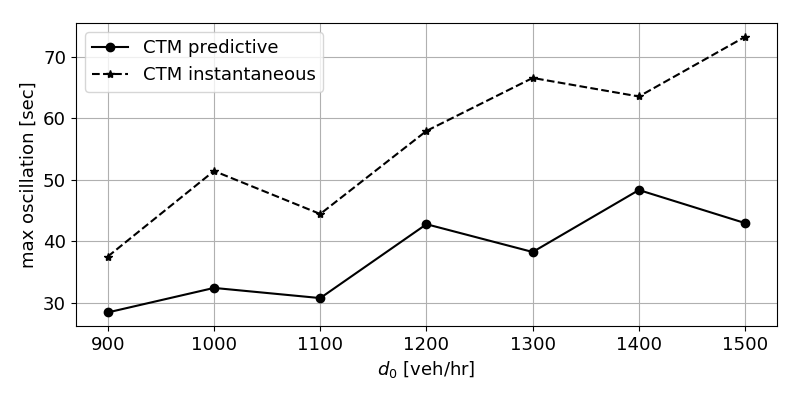
\includegraphics[width=\linewidth]{figs/peaks.png}
    \caption{\XXX }
    \label{fig:peaks}
\end{figure}

% \begin{figure}[h]
%     \centering
%     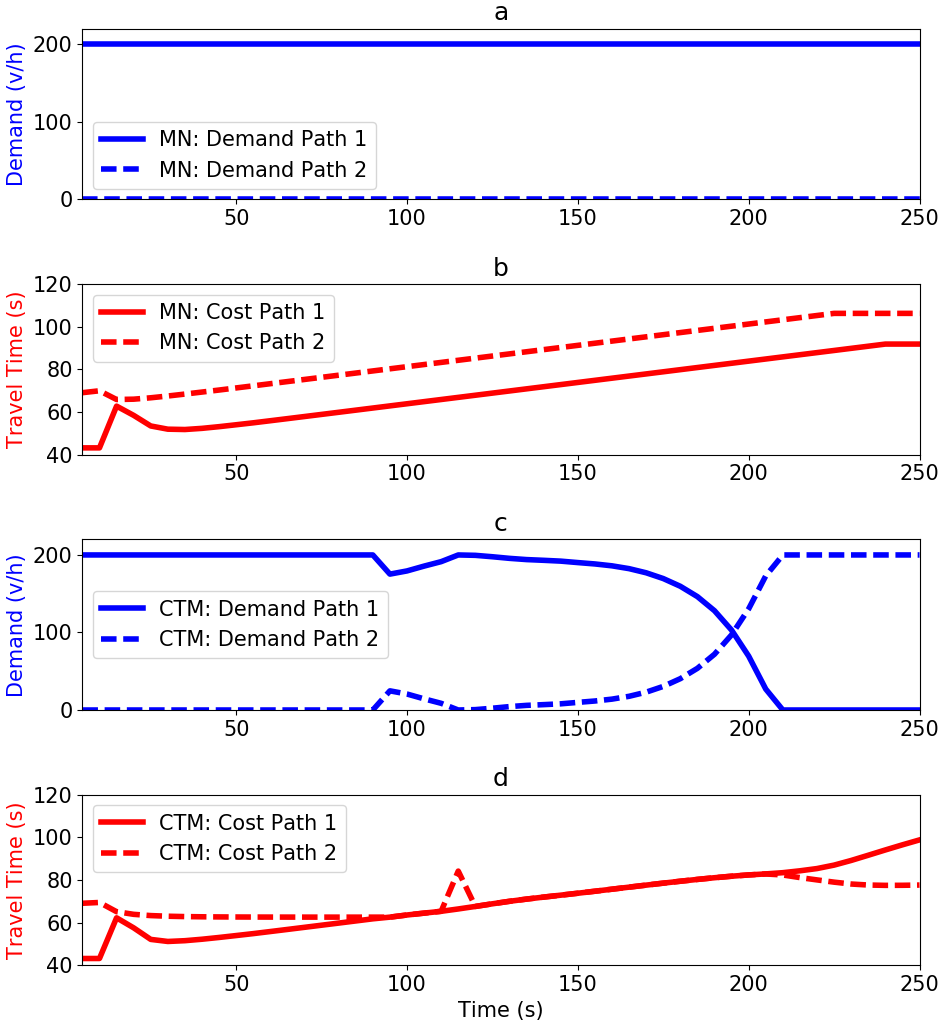
\includegraphics[width=\linewidth]{figs/Paper_dta_results_mn_ctm.PNG}
%     \caption{a. MN Equilibrium Assignment on Path 1 and 2 b. MN Travel Time on Path 1 and 2 c. CTM Equilibrium Assignment on Path 1 and 2 d. CTM Travel Time on Path 1 and 2 }
%     \label{fig:DTA_Results}
% \end{figure}

